%%%%%%%%%%%%%%%%%%%%%%%%%%%%%%%%%%%%%%%%%%%%%%%%%%%%%%%%%%%%%%%%%%%%%
% LaTeX Template: Praxisprojekt WS 2017
%
% Date: November 2017
%
%%%%%%%%%%%%%%%%%%%%%%%%%%%%%%%%%%%%%%%%%%%%%%%%%%%%%%%%%%%%%%%%%%%%%%

\documentclass[12pt]{article}
\usepackage[a4paper]{geometry}
\usepackage{framed}
\usepackage[myheadings]{fullpage}
\usepackage{fancyhdr}
\usepackage{lastpage}
\usepackage{graphicx, wrapfig, subcaption, setspace, booktabs}
\usepackage[T1]{fontenc}
\usepackage[font=small, labelfont=bf]{caption}
\usepackage[protrusion=true, expansion=true]{microtype}
\usepackage[german]{babel}
\usepackage{sectsty}
\usepackage{url, lipsum}
\usepackage[parfill]{parskip}
\usepackage{listings}
\usepackage{svg}
\usepackage{amsmath}


\usepackage{enumitem,amssymb}
\newlist{todolist}{itemize}{2}
\setlist[todolist]{label=$\square$}
\usepackage{pifont}
\newcommand{\cmark}{\ding{51}}%
\newcommand{\xmark}{\ding{55}}%
\newcommand{\done}{\rlap{$\square$}{\raisebox{2pt}{\large\hspace{1pt}\cmark}}%
\hspace{-2.5pt}}
\newcommand{\wontfix}{\rlap{$\square$}{\large\hspace{1pt}\xmark}}

\usepackage{dirtree}
\DTsetlength{ 0.2em}{ 1em}{ 0.2em}{ 0.4pt}{ 0.1pt}

%-------------------------------------------------------------------------------
% Commands
%-------------------------------------------------------------------------------
\newcommand{\HRule}[1]{\rule{\linewidth}{#1}}
\input{env}
%-------------------------------------------------------------------------------
% HEADER & FOOTER
%-------------------------------------------------------------------------------
\pagestyle{fancy}
\fancyhf{}
\setlength\headheight{15pt}
\fancyhead[L]{\newCommandName}
\fancyhead[R]{\newCommandUniversity}
\fancyfoot[R]{Seite \thepage\ von \pageref{LastPage}}

%-------------------------------------------------------------------------------
% TITLE PAGE
%-------------------------------------------------------------------------------
\begin{document}


\title{ \normalsize
		\HRule{0.5pt} \\
		\LARGE \textbf{\uppercase{\newCommandDiscipline}} \\
		\smallbreak
		\small\textbf{{\newCommandTerm}}\\
		\HRule{2pt} \\ [0.5cm]
		\normalsize \today \vspace*{10\baselineskip}}

\date{}

\author{
		\newCommandName \\
		\newCommandMatriculationNumber \\
		\newCommandUniversity \\
		\newCommandFaculty
}

\pagenumbering{gobble}

\maketitle

\newpage

\pagenumbering{arabic}


%-------------------------------------------------------------------------------
% Section title formatting
\sectionfont{\scshape}
%-------------------------------------------------------------------------------

%-------------------------------------------------------------------------------
% BODY
%-------------------------------------------------------------------------------

\section{Statusbericht}
\subsection{Was habe ich bisher im Projekt erreicht?}
\begin{itemize}
	\item Rest-Crud Api f"ur Jobs abgeschlossen
	\begin{figure}[!htp]
		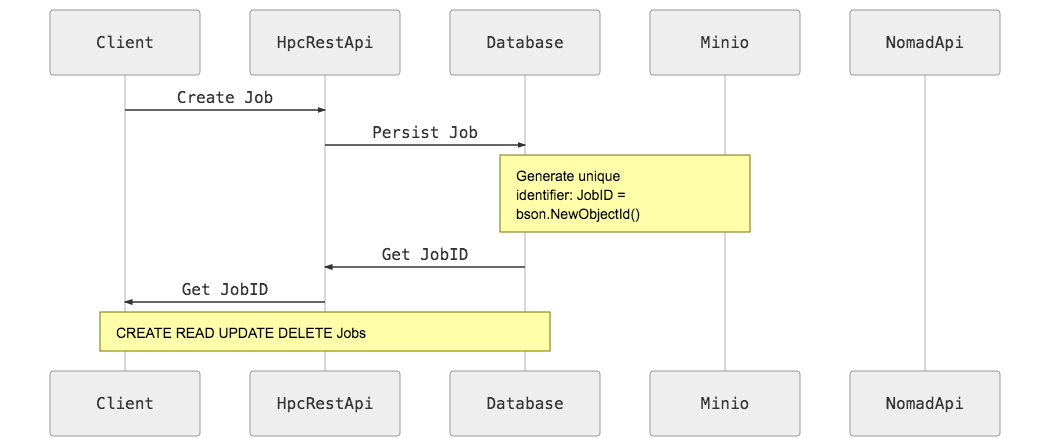
\includegraphics[width=1\textwidth]{./img/01_create-job.png}
		\captionsetup{name=Abb.,font=footnotesize}
		\caption{Rest-Crud Api f"ur Jobs}
		% \centering
	\end{figure}
	\item Rest-Crud Api f"ur Templates(Varianten) abgeschlossen
	\begin{figure}[!htp]
		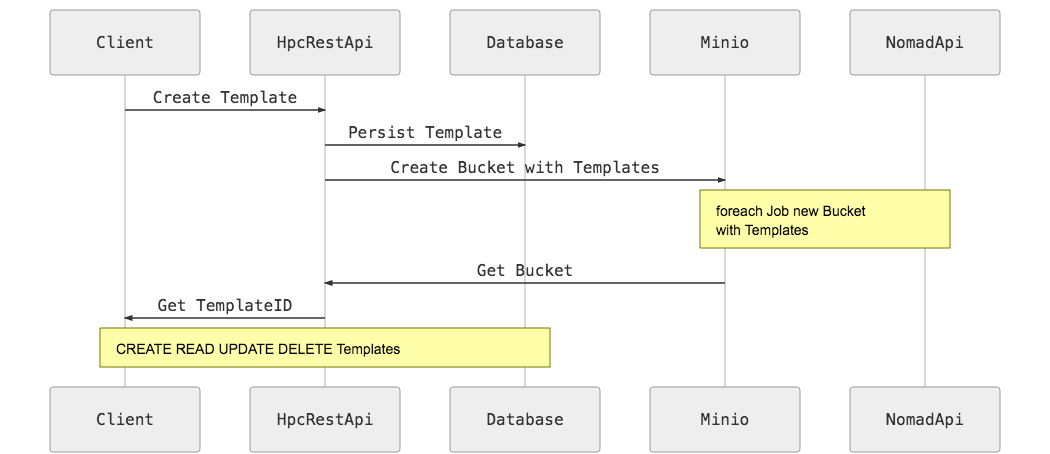
\includegraphics[width=1\textwidth]{./img/02_create-template.png}
		\captionsetup{name=Abb.,font=footnotesize}
		\caption{Rest-Crud Api f"ur Templates}
		% \centering
	\end{figure}
	\item Datenbank-Persistenz (MongoDB)
	\item Templates werden angelegt und es werden Json-Template gerendert und im Objectstore (Minio) abgelegt
	\item Job-Submit - Jobs werden submitted an Nomad

\end{itemize}
\smallbreak


\subsection{Was habe ich bis zum n"achsten Statusbericht vor?}
\begin{itemize}
\item Notification Job Finished
\item Write back Job-Result to Minio
\begin{figure}[!htp]
	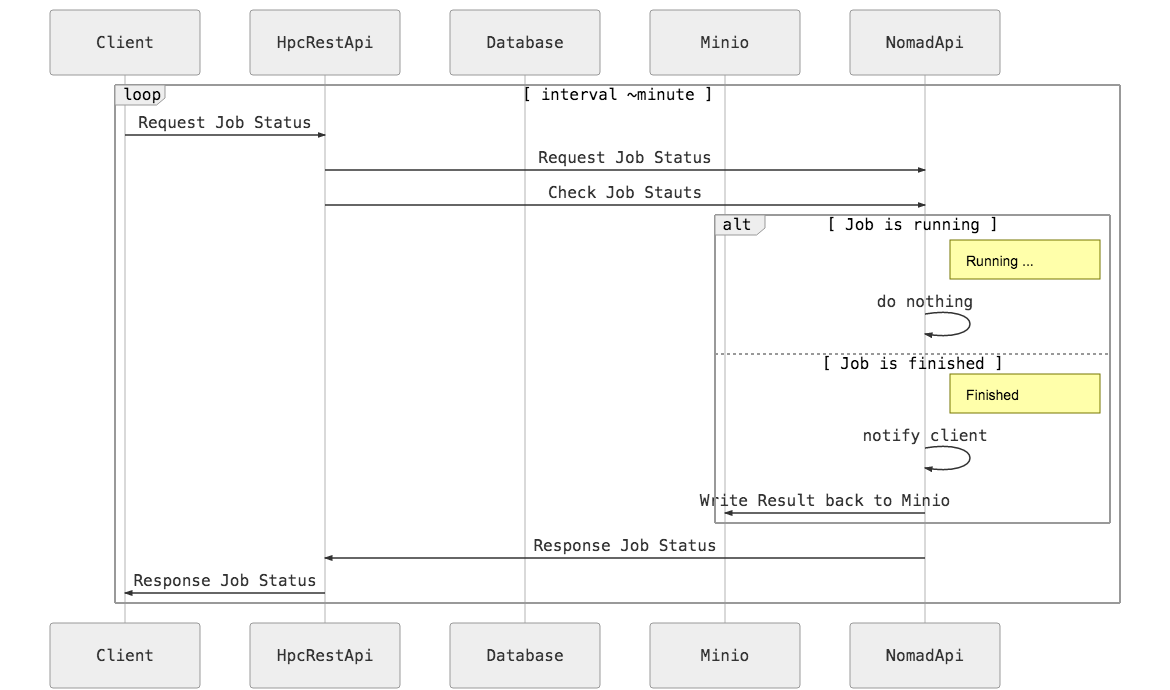
\includegraphics[width=1\textwidth]{./img/03_client-get-job-status.png}
	\captionsetup{name=Abb.,font=footnotesize}
	\caption{Client get Job-Status - Write Result back and notify the Client}
	% \centering
\end{figure}
\item Dokumentation
\item Dockerizing des Stacks (MongoDB, Minio, Nomad) mit Docker-Compose
\end{itemize}

Dokumentation der Issues werden direkt im Repository gef"uhrt.
\subsection{Gibt es Probleme bei der Durchf"uhrung?}
\begin{itemize}
\item Es ist momentan noch unklar wie der Client benachrichtigt wird wenn die Jobs beendet sind.
\item Es ist momentan noch unklar wie die Results der Jobs zur"uckgeschrieben werden.
\end{itemize}


\section{Ressourcen}
\textbf{Git-Repository als Versionskontrolle:}\\
\url{https://github.com/MatthiasHertel/ws17_pp}

\textbf{Webseite zur Dokumentation:}\\
\url{https://www.ws17-pp.mhertel.de}


\end{document}
